\documentclass[12pt,a4paper]{report}
\usepackage[utf8]{inputenc}
\usepackage[T1]{fontenc}
\usepackage[french]{babel}
\usepackage{geometry}
\usepackage{graphicx}
\usepackage{caption}
\usepackage{subcaption}
\usepackage{float}
\usepackage{lmodern}
\usepackage{setspace}
\usepackage{fancyhdr}
\pagestyle{fancy}
\usepackage{amsmath}
\usepackage{enumitem}
\usepackage{url}
\usepackage{xurl}

% Corriger ce que contient \leftmark pour les chapitres
\renewcommand{\chaptermark}[1]{%
  \markboth{CHAPITRE \thechapter. \ #1}{}%
}

\fancyhf{} % Réinitialise tout
\fancyhead[L]{\nouppercase{\leftmark}} % Titre du chapitre
\fancyfoot[L]{Evan Combot}
\fancyfoot[C]{\thepage}
\fancyfoot[R]{Université de Montpellier}

% Appliquer aussi aux pages de style "plain"
\fancypagestyle{plain}{%
  \fancyhf{}
  \fancyhead[L]{\nouppercase{\leftmark}}
  \fancyfoot[L]{Evan COMBOT}
  \fancyfoot[C]{\thepage}
  \fancyfoot[R]{Université de Montpellier}
}

\usepackage{titling}
\usepackage{mathpazo}
\usepackage{ragged2e}
\usepackage{titlesec}
\titleformat{\chapter}[display]{\normalfont\huge\bfseries}{\chaptername\ \thechapter}{10pt}{\Huge}
\titlespacing*{\chapter}{0pt}{-20pt}{30pt}
\setcounter{secnumdepth}{6}

% === Pour gérer les marges58 ===
\geometry{left=2.0cm, right=2.0cm, top=2.0cm, bottom=2.0cm}
\onehalfspacing
\usepackage[]{hyperref}

\titleformat{\subsubsection}[block]{\bfseries\Large}{\thesubsubsection}{1em}{}
\titleformat{\paragraph}[block]{\bfseries\large}{\theparagraph}{1em}{}
\titleformat{\subparagraph}[block]{\bfseries\normalsize}{\thesubparagraph}{1em}{}

\begin{document}
\justifying

\begin{titlepage}
\begin{center}

% === LOGOS ALIGNÉS EN LIGNE AVEC LÉGENDES EN GRAS ===
\vspace*{0.5cm}
\begin{minipage}{0.3\textwidth}
    \centering
    
\includegraphics[width=0.85\textwidth]{Assets/UM.png}\\[0.2cm]
    {\footnotesize\textbf{Université de Montpellier}}
\end{minipage}
\hfill
\begin{minipage}{0.3\textwidth}
    \centering
    
\includegraphics[width=0.85\textwidth]{Assets/Dpt_Info.png}\\[0.2cm]
    {\footnotesize\textbf{Département Informatique -- IMAGINE}}
\end{minipage}
\hfill
\begin{minipage}{0.3\textwidth}
    \centering
    
\includegraphics[width=0.85\textwidth]{Assets/CEA.png}\\[0.2cm]
    {\footnotesize\textbf{CEA -- Commissariat à l'énergie atomique et aux énergies alternatives}}
\end{minipage}

\vspace{1.8cm}

% === ÉTABLISSEMENT & DIPLÔME ===
{\Large \textbf{Université de Montpellier}}\\[0.2cm]
{\normalsize Faculté des Sciences}\\[0.3cm]
{\large \textbf{Master 2 Informatique -- Parcours \og IMAGINE \fg{}}}\\[1.5cm]

% === TITRE DU DOCUMENT ===
{\Huge \bfseries Rapport de Stage}\\[0.4cm]
\rule{0.65\linewidth}{0.7pt}\\[1cm]

{\large \textbf{Exploitation d'images de caractérisation de chaîne radiographique}}\\[0.5cm]
\textit{Stage réalisé au sein du \textbf{Commissariat à l'énergie atomique et aux énergies alternatives}}\\[0.3cm]
\textit{du \textbf{3 février 2025} au \textbf{1 août 2025}}\\[2cm]

% === INFOS ÉTUDIANT & ENTREPRISE ===
\begin{flushleft}
\textbf{Réalisé par :} \hfill COMBOT Evan\\[0.15cm]
\textbf{Année universitaire :} \hfill 2024--2025\\[0.15cm]
\textbf{Tuteur en entreprise :} \hfill Nom Prénom\\[0.15cm]
\textbf{Encadrant pédagogique :} \hfill PUECH William\\[0.15cm]
\textbf{Adresse de l'entreprise :} \hfill CEA Gramat, 46500 Gramat, France
\end{flushleft}

\vfill
{\small Date de rendu : 20 juin 2025}

\end{center}
\end{titlepage}

%======================
% Remerciements
%======================
\chapter*{Remerciements}
\addcontentsline{toc}{chapter}{Remerciements}

Je souhaite exprimer ma profonde gratitude à toutes les personnes qui m'ont soutenu(e) et accompagné(e) tout au long de ce stage.

Je remercie tout particulièrement :
\begin{itemize}
  \item M. Nom Prénom, mon tuteur de stage en entreprise, pour son accueil chaleureux, son encadrement attentif et sa grande disponibilité ;
  \item M. William Puech, mon encadrant pédagogique, pour son suivi rigoureux et sa bienveillance;
  \item Je remercie toute l’équipe du CEA pour son soutien constant, sa convivialité, l’excellente ambiance de travail qu’elle a su instaurer, ainsi que pour m’avoir intégré(e) avec tant de rapidité et de bienveillance.
\end{itemize}

Je tiens également à exprimer ma gratitude envers l’ensemble des enseignants du Master 2 IMAGINE pour la qualité de leur enseignement et les compétences précieuses qu’ils m’ont transmises tout au long de la formation, et qui me sont aujourd’hui particulièrement utiles.

\tableofcontents
\pagestyle{fancy}
\newpage

\chapter{Introduction}

Ce chapitre vise à présenter le cadre dans lequel s’inscrit ce stage ainsi que les objectifs poursuivis dans le présent rapport. Il fournit les éléments de contexte nécessaires à la compréhension du travail réalisé et introduit la structure adoptée pour en rendre compte.

\section{Contexte du stage}
Le stage s’est déroulé au sein du Commissariat à l'Énergie Atomique et aux Énergies Alternatives (CEA), un organisme public de recherche de renommée internationale, intervenant dans les domaines de l’énergie, de la défense, des technologies de l’information et de la santé. Il s’inscrit dans le cadre du Master IMAGINE, une formation axée sur le traitement d’images, la 3D et l’intelligence artificielle. Ce stage de fin d’études avait pour objectif de mettre en pratique les compétences acquises tout au long de la formation, en contribuant au développement d’outils à vocation principalement applicative, intégrant également une dimension de recherche, dans le domaine de l’imagerie radiographique.

\section{Objectifs du rapport}
L’objectif de ce rapport est de rendre compte du stage effectué à travers :

\begin{itemize}
\item La présentation du cadre et des objectifs de la mission ;
\item La description des tâches réalisées et des méthodes employées ;
\item La mise en avant des outils et technologies utilisés ;
\item L’analyse des difficultés rencontrées et des solutions apportées ;
\item Un bilan des compétences acquises, tant sur le plan technique que personnel.
\end{itemize}

Ce rapport vise également à illustrer l'application concrète des connaissances acquises durant la formation.

\chapter{Présentation de l'entreprise}
Ce chapitre a pour but de présenter l’organisme qui m’a accueilli durant mon stage. J’y expose brièvement son historique, ses principales missions et son organisation générale. Une attention particulière est accordée à la Direction des Applications Militaires, au sein de laquelle j’ai eu l’opportunité d’effectuer ma mission.

\section{Le Commissariat à l'énergie atomique et aux énergies alternatives}
\subsection{Historique}

Le Commissariat à l’énergie atomique (CEA) a été créé en 1945, à l’initiative du général de Gaulle, dans un contexte où les avancées sur la radioactivité et la fission nucléaire ouvraient la voie à des applications civiles et militaires majeures. Cette décision s’inscrivait dans la continuité des découvertes de scientifiques comme Henri Becquerel, Pierre et Marie Curie, ou encore Irène et Frédéric Joliot-Curie. En 2009, pour refléter l’élargissement de ses missions aux énergies renouvelables, l’organisme prend le nom de \textit{Commissariat à l'énergie atomique et aux énergies alternatives (CEA)}.

\subsection{Activités}
Actuellement, le \textit{Commissariat à l'énergie atomique et aux énergies alternatives (CEA)} est structuré autour de quatre grandes directions opérationnelles :

\begin{itemize} \item \textbf{La Direction des énergies (DES)} : mène des recherches sur l’énergie nucléaire civile, les systèmes énergétiques innovants et la transition énergétique.

\item \textbf{La Direction des applications militaires (DAM)} : assure les missions de défense nationale, notamment la dissuasion nucléaire et la sécurité des installations.

\item \textbf{La Direction de la recherche technologique (DRT)} : développe des innovations technologiques et des partenariats industriels, notamment dans la microélectronique, les systèmes intelligents et les énergies renouvelables.

\item \textbf{La Direction de la recherche fondamentale (DRF)} : explore les sciences fondamentales, telles que la physique nucléaire, la biologie, la climatologie et les sciences de l’univers. \end{itemize}

\subsection{Organisation}
Aujourd'hui, le CEA est composé de neuf centres de recherche, dont certains sont placés sous la responsabilité de la \textit{Direction des applications militaires (DAM)} pour des missions de défense, tandis que d'autres sont dédiés aux applications civiles. Il regroupe également cinquante-deux unités mixtes de recherche (UMR), a déposé 725 brevets prioritaires, dispose de vingt-six équipements d’excellence (Équipex) et de seize laboratoires d’excellence (Labex). En 2023, le CEA comptait un effectif total de 16 564 employés.

\section{La Direction des Applications Militaires}
\subsection{Historique \& activités}
La Direction des applications militaires (DAM) a été créée secrètement en 1955 sous le nom de \textit{Bureau d'études générales (BEG)}. Ce n'est qu'en 1958 que le général de Gaulle officialise la création de la DAM au sein du Commissariat à l'énergie atomique (CEA). Les armes nucléaires, les réacteurs nucléaires pour la propulsion navale et les matières nucléaires stratégiques constituent le cœur de sa mission, centrée sur la dissuasion nucléaire française. Aujourd'hui, la DAM contribue à l'excellence de la recherche, renforce la compétitivité industrielle, assure la surveillance, l'analyse et l'intervention pour la défense et la sécurité nationale, tout en répondant aux enjeux liés à la dissuasion nucléaire. En 2023, elle comptait près de 4 802 employés.
\subsection{Le centre de Bruyères-le-Châtel}
Le centre de Bruyères-le-Châtel, connu sous le nom de \textit{CEA-DIF} ou par son nom de code \textit{BIII} (B3), regroupe près de 2 000 ingénieurs, chercheurs et techniciens. Ils conçoivent les réacteurs nucléaires des sous-marins français et du porte-avions \textit{Charles de Gaulle}, ainsi que les armes nucléaires françaises, en s’appuyant notamment sur le programme \textit{Simulation}. Le centre participe également à la lutte contre la prolifération et le terrorisme nucléaire.
Premier site officiel de la \textit{Direction des applications militaires (DAM)}, sous le code \textit{BIII}, c’est sur ce site qu’a été conçue la première bombe atomique française, \textit{Gerboise Bleue}. Le centre aurait par ailleurs fabriqué plus de 90 \% des armes nucléaires testées lors des essais français au Sahara et dans le Pacifique.

\chapter{Présentation de la mission}

Ce chapitre vise à présenter le cadre dans lequel s’est inscrite ma mission de stage. Il introduit d’abord le programme \textit{Simulation} auquel mon projet est rattaché, puis détaille les enjeux techniques et scientifiques, ainsi que les objectifs définis en début de stage.

\section{Contexte de la mission}
 Dans un contexte d'amélioration et de refactorisation de codes précédents, l'objectif principal de ma stage a été de .... .Cette modélisation permettra de ...


Exemple ! : Au CEA, mon travail s'est inscrit dans une démarche d'innovation visant à modéliser une chaîne radiographique complète. Cette modélisation a pour ambition de mieux comprendre le comportement du système d'imagerie, d'optimiser ses performances et d'améliorer la qualité des images obtenues, tout en respectant les contraintes liées à la radioprotection.

Le stage a ainsi offert un cadre idéal pour mettre en pratique des compétences en physique médicale, traitement du signal et programmation, au service d'une problématique appliquée et concrète.


Contexte professionnel de ta mission, ce que tu devais faire, les enjeux, la méthodologie, les objectifs pratiques.

qui s'incrit dans le programme Simulation

\subsection{Le programme Simulation}
Lancé en 1995, le programme Simulation vise à pérenniser la dissuasion nucléaire française à la suite de l’arrêt définitif des essais nucléaires. Il a été conçu pour garantir, dans la durée, la fiabilité, la sûreté et la performance des armes qui composent les deux volets de la dissuasion nucléaire nationale. Ce programme répond également à un enjeu stratégique : maintenir les compétences scientifiques et techniques dans un domaine aussi complexe que sensible, en assurant la formation de nouveaux experts dans le domaine très spécialisé du fonctionnement des armes nucléaires.

Le programme Simulation repose sur une démarche scientifique rigoureuse et se structure autour de trois piliers complémentaires :
\renewcommand{\labelitemi}{$\bullet$}
\begin{itemize}
\item \textbf{La physique des armes} : elle consiste à modéliser l'ensemble des phénomènes physiques intervenant dans le fonctionnement d'une arme nucléaire. Cela implique de concevoir, sélectionner et enchaîner des modèles physiques pour reproduire par le calcul les trois phases majeures : pyrotechnique, fission, puis fusion. Ces modèles sont intégrés dans un système d’équations mathématiques complexes visant à simuler le comportement réel de l’arme avec la plus grande précision possible. Parmi les disciplines mobilisées figurent la mécanique des fluides, la neutronique (calcul des flux de neutrons), la dynamique de la matière et le transport des photons.
\begin{figure}[H]
    \centering % <--- ici pour tout centrer
    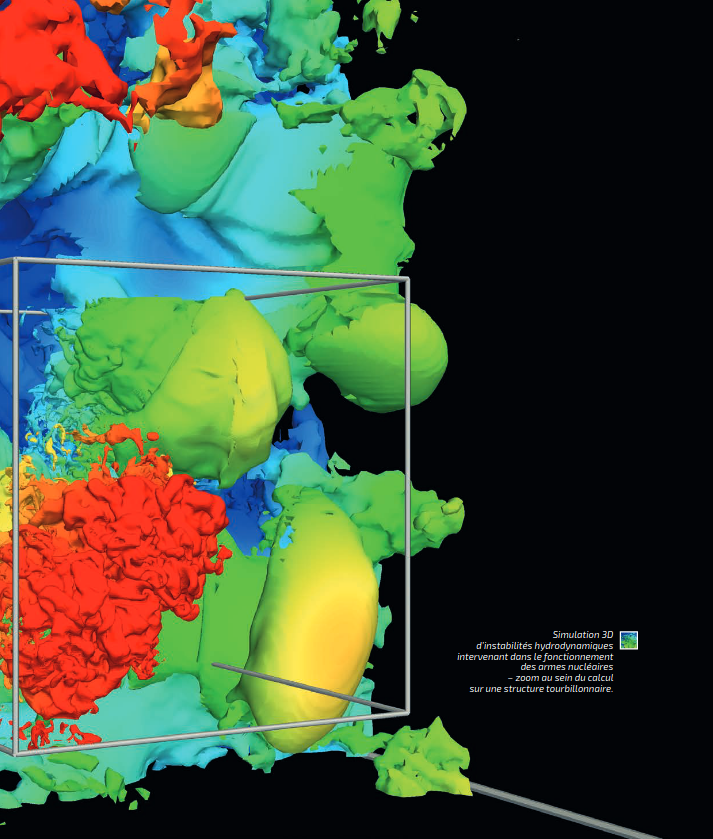
\includegraphics[height=5cm]{Assets/Physique_arme.png}
        %\caption{Liaisons entre les classes du moteur}
\end{figure}

\item \textbf{La simulation numérique} : elle permet de reproduire virtuellement le fonctionnement des armes grâce à des calculs intensifs réalisés sur des modèles numériques. La modélisation d’une arme nucléaire nécessite de mailler finement l’espace simulé, avec parfois plusieurs centaines de millions de mailles, ce qui engendre des systèmes d’équations comportant plusieurs milliards d’inconnues. Pour résoudre ces équations dans un délai raisonnable, des supercalculateurs de plus en plus puissants ont été développés. Trois générations ont été successivement mises en œuvre : TERA 1 (2001, 5 teraflops), TERA 10 (2005, 50 teraflops), et TERA 100 (2010, 1,3 petaflops).

\begin{figure}[H]
    \hspace{0cm} % <<== Décale tout vers la gauche
    \begin{subfigure}[t]{0.42\textwidth}
        \centering
        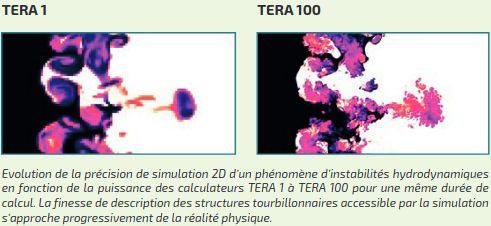
\includegraphics[height=5cm]{Assets/Exemple_Simulation.png}
        \caption{Liaisons entre les classes du moteur}
    \end{subfigure}
    \hspace{10em} % <<== Espace entre les deux images
    \begin{subfigure}[t]{0.42\textwidth}
        \centering
        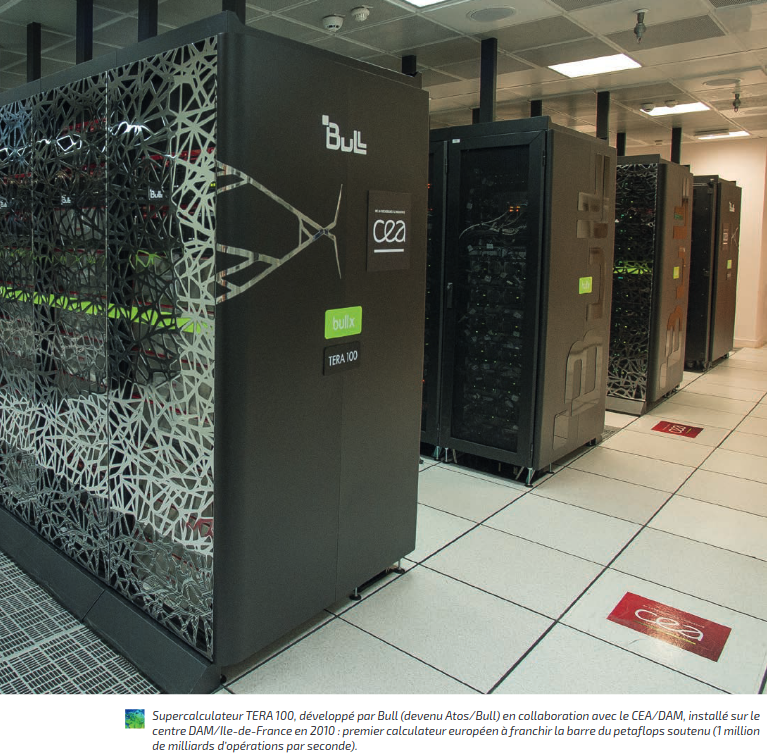
\includegraphics[height=5cm]{Assets/Supercalculateur.png}
        \caption{Supercalculateur utilisé pour les simulations}
    \end{subfigure}
    \caption{Illustrations du fonctionnement du programme Simulation}
    \label{fig:images}
\end{figure}

\item \textbf{La validation expérimentale} : cette phase permet de confronter les résultats des simulations à des données expérimentales. Deux installations majeures y contribuent. L’installation EPURE, dédiée à la radiographie, permet d’observer la phase non nucléaire du fonctionnement de l’arme avec une extrême précision. Quant au Laser Mégajoule, il s’agit d’un laser de très grande puissance, capable de recréer à une échelle réduite les conditions extrêmes de température et de pression rencontrées lors des réactions nucléaires. Ces deux installations sont essentielles pour garantir la crédibilité scientifique et technique des simulations effectuées.
\end{itemize}

\section{Enjeux et objectifs}
Les tâches que je réalise ont pour termes ... des compute mass image ...


\chapter{Environnement technique}

Ce chapitre décrit l’environnement technique dans lequel s’est déroulé mon stage au CEA. J’y présente les principales technologies mobilisées, les outils de développement utilisés au quotidien, ainsi que les contraintes spécifiques — qu’elles soient techniques, sécuritaires ou organisationnelles liées au contexte de travail.

\section{Technologies utilisées}
... % à compléter

\section{Outils de développement}
... % à compléter

\section{Contraintes techniques}
... % à compléter

\chapter{Veille technologique}
Dans le cadre de ce stage, il m’a été essentiel de consolider et d’approfondir certaines bases scientifiques et techniques afin de mieux comprendre les outils et phénomènes physiques impliqués dans la mission. En effet, une bonne compréhension des principes de fonctionnement des machines de radiographie, ainsi que des phénomènes physiques associés à la propagation des ondes (en particulier les rayons X et les neutrons), est indispensable pour appréhender correctement les étapes de traitement d’images et de données.

Cette veille technologique a donc permis de :
\begin{itemize}
  \item Consolider les bases de la physique des rayonnements ionisants, notamment en ce qui concerne la nature et l’interaction des rayons X et des neutrons avec la matière ;
  \item Comprendre le fonctionnement des machines de radiographie à haute énergie utilisées sur l’installation EPURE ;
  \item Relier les phénomènes physiques fondamentaux (effet photoélectrique, diffusion Compton, production de paires) aux caractéristiques des images radiographiques obtenues ;
  \item Appréhender les principes de détection des rayonnements ainsi que les choix technologiques associés (détecteurs directs et indirects, CCD, gamma-caméra, scintillateurs) ;
  \item Acquérir une première maîtrise des techniques de traitement d’image appliquées aux radiographies dynamiques de haute énergie.
\end{itemize}

Cette base théorique et technique constitue un socle indispensable pour comprendre le travail réalisé durant le stage, notamment la modélisation de chaînes radiographiques, l’analyse des performances des dispositifs de détection, et l’étude des algorithmes d’extraction d’information physique à partir des images acquises. Les sections suivantes présentent de manière structurée les principaux éléments étudiés dans ce cadre.

\section{Modélisation d'une chaîne radiographique}
\subsection{Nature du rayonnement électromagnétique}
Une onde électromagnétique est le résultat de l’oscillation synchronisée d’un champ électrique et d’un champ magnétique, chacun étant perpendiculaire à l’autre ainsi qu’à la direction de propagation. Dans le vide, cette onde se déplace à la vitesse de la lumière, notée $c = 299,792,458 , \text{m/s}$. Lorsqu’il s’agit d’une onde monochromatique, sa fréquence $\nu$ et sa période $T$ sont reliées par $T = 1/\nu$. Sa longueur d’onde $\lambda$ correspond à la distance parcourue pendant une période, soit $\lambda = c T = c/\nu$.

En pratique, les ondes électromagnétiques observées sont souvent des superpositions de fréquences multiples, formant un spectre. Ce spectre décrit la répartition de l’énergie en fonction de la fréquence ou de la longueur d’onde. Les ondes sont classées selon leur domaine spectral : on distingue ainsi les ondes radio, les micro-ondes, l’infrarouge, la lumière visible, l’ultraviolet, les rayons X et les rayons gamma. Bien que de même nature, ces ondes diffèrent par leurs mécanismes d’émission, d’interaction avec la matière et par les capteurs nécessaires à leur détection.
\begin{figure}[H]
    \centering
    \includegraphics[height=7cm]{Assets/Spectre_Electro.png}
    \caption{Spectre électromagnétique}
    \label{fig:images}
\end{figure}

\subsection{Imagerie par rayons X}
Les rayons X, situés dans une gamme de fréquences allant de $10^{16}$ Hz à $10^{20}$ Hz, sont des ondes électromagnétiques particulièrement énergétiques. Ils sont générés artificiellement à l’aide de dispositifs appelés tubes à rayons X, tels que les tubes de Coolidge. Dans ces tubes, des électrons émis par une cathode sont accélérés par une tension élevée, puis projetés contre une cible métallique. Le freinage brutal des électrons dans cette cible engendre un rayonnement continu (appelé Bremsstrahlung), complété par des raies caractéristiques dépendant de la nature du matériau.

Ces rayons interagissent avec les matériaux traversés, principalement par absorption. Les différences d’atténuation selon les structures traversées permettent de former des images révélant les contrastes de densité et de composition des objets.

\begin{figure}[H]
    \centering
    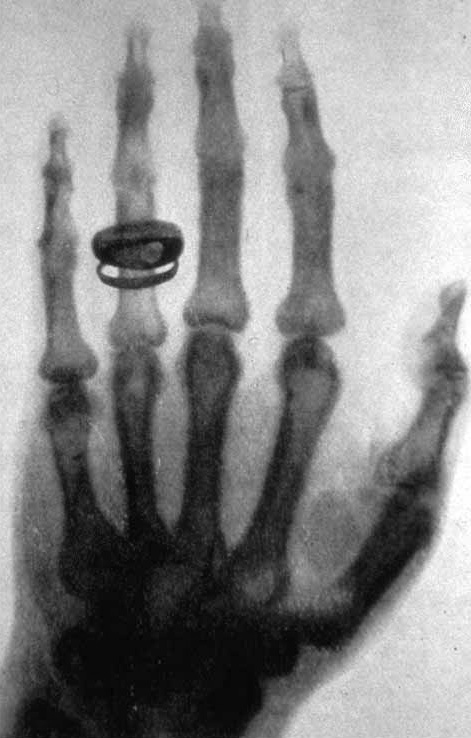
\includegraphics[height=7cm]{Assets/Exemple_xray.png}
    \caption{Exemple d'une image obtenue à partir de rayons X}
    \label{fig:images}
\end{figure}

\subsection{Imagerie neutronique}
L’imagerie neutronique repose sur des principes analogues à ceux de la radiographie X, mais utilise un autre type de rayonnement : les neutrons. Contrairement aux photons, les neutrons interagissent principalement avec les noyaux des atomes et non avec les électrons. Cette différence d’interaction offre une complémentarité précieuse : là où les rayons X sont fortement atténués par les matériaux lourds, les neutrons peuvent les traverser plus aisément tout en étant sensibles à des éléments légers comme l’hydrogène, le bore ou le lithium.

Cependant, produire un flux de neutrons suffisamment intense et collimaté pour l’imagerie nécessite des installations lourdes (générateurs, réacteurs expérimentaux), ce qui limite leur emploi à des applications industrielles ou scientifiques spécialisées.
\begin{figure}[H]
    \centering
    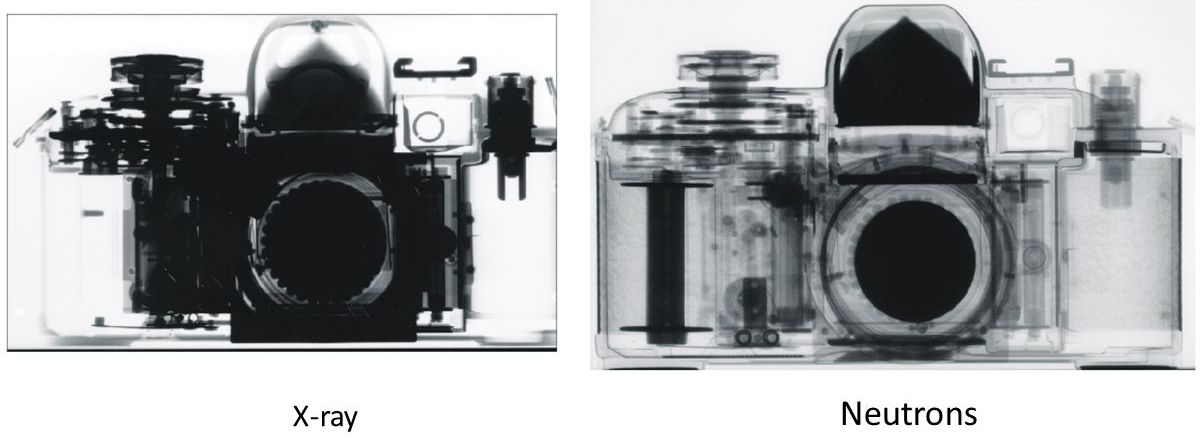
\includegraphics[height=5cm]{Assets/Imagerie_neutron_xray.png}
    \caption{Comparaison entre l'imagerie rayons X (gauche) et l'imagerie neutronique (droite)}
    \label{fig:images}
\end{figure}

\section{Fonctionnement détaillé de la chaîne radiographique}
Maintenant que les principales méthodes d’imagerie ont été présentées, il convient de s’intéresser au fonctionnement global d’une chaîne radiographique, en mettant l’accent sur sa modélisation.

\subsection{Production des rayons X}
Dans une chaîne radiographique, les rayons X peuvent être générés par deux types de sources :
\begin{itemize}
\item des \textbf{tubes à rayons X}, où l’accélération d’électrons est assurée par une tension fixe (jusqu’à 150 kV) ;
\item des \textbf{accélérateurs à induction} ou linéaires (LINAC), capables de produire des faisceaux d’électrons relativistes (jusqu’à plusieurs dizaines de MeV), comme c’est le cas pour les installations telles qu’Airix.
\end{itemize}
Dans les deux cas, l’impact des électrons sur une cible métallique engendre l’émission de rayons X selon deux mécanismes :
\begin{itemize}
\item \textit{Rayonnement de freinage} (Bremsstrahlung), qui produit un spectre continu ;
\item \textit{Rayonnement caractéristique}, lié aux réarrangements électroniques internes des atomes de la cible.
\end{itemize}
\begin{figure}[H]
    \centering
    \includegraphics[height=7cm]{Assets/Tube_rayons_X.png}
    \caption{Tube à rayons X}
    \label{fig:images}
\end{figure}

\subsection{Interactions rayonnement/matière}
Les photons X peuvent interagir avec les atomes des matériaux traversés via plusieurs processus :
\begin{itemize}
\item \textbf{Effet photoélectrique} : un photon est totalement absorbé, ce qui provoque l’éjection d’un électron d’une couche interne ;
\item \textbf{Diffusion Compton} : le photon est diffusé en perdant une partie de son énergie au profit d’un électron faiblement lié ;
\item \textbf{Production de paires} : si l’énergie du photon est supérieure à 1,022 MeV, il peut se matérialiser en un électron et un positon.
\end{itemize}
L’intensité du rayonnement transmis diminue exponentiellement avec la distance $z$ traversée dans un matériau, selon la loi $N(z) = N_0 e^{-\mu z}$, où $\mu$ est le coefficient d’atténuation massique dépendant de la nature du matériau et de l’énergie du photon.

\subsection{Détection des rayonnements}
\paragraph{Principe général} La détection vise à convertir l’énergie déposée par les rayons X dans un capteur en un signal électrique mesurable. Deux grands types de détecteurs se distinguent :
\begin{itemize}
\item \textbf{Détecteurs indirects} : ils utilisent un scintillateur qui transforme les photons X en lumière visible, laquelle est ensuite captée par un capteur optique (CCD, CMOS, photodiode).
\item \textbf{Détecteurs directs} : les photons sont convertis directement en charges électriques dans un semi-conducteur (ex. : CdTe, a-Se), permettant une résolution spatiale supérieure et une meilleure efficacité de détection.
\end{itemize}

\paragraph{Paramètres de performance} Les détecteurs sont évalués selon plusieurs critères :
\begin{itemize}
\item la \textbf{résolution spatiale}, qui mesure la finesse des détails visibles ;
\item le \textbf{seuil de détection}, définissant la plus faible quantité de rayonnement détectable ;
\item la \textbf{réponse en dose}, c’est-à-dire la linéarité entre l’intensité du signal et la dose reçue ;
\item le \textbf{rapport signal/bruit} (SNR) et l’\textbf{efficacité quantique de détection} (DQE), qui caractérisent la qualité globale de l’image obtenue.
\end{itemize}

\subsection{Traitement des images}
L’image acquise par la chaîne radiographique est une projection 2D de l’atténuation du rayonnement à travers l’objet. Pour en extraire une information exploitable, plusieurs étapes de traitement sont nécessaires :
\begin{itemize}
\item \textbf{Correction des non-linéarités} liées au détecteur, via des calibrations effectuées sur des maquettes étalon aux propriétés connues ;
\item \textbf{Filtrage et restauration d’image}, pour compenser le bruit et le flou (liés au mouvement, à la diffusion, ou à la largeur de la source) ;
\item \textbf{Reconstruction de la masse surfacique}, voire de la densité volumique dans le cas de mesures multi-angles (tomographie).
\end{itemize}

\section{Principe de fonctionnement de l'installation EPURE}
L’installation EPURE (Explosions pour l’Utilisation et la Recherche Expérimentale) est une infrastructure franco-britannique localisée à Valduc, dédiée aux expérimentations hydrodynamiques avec radiographie éclair. Elle s’inscrit dans le cadre du programme Simulation, qui permet de garantir la sûreté et la fiabilité des armements nucléaires sans recours à des essais réels. Cette installation a pour objectif de capturer, avec une extrême précision temporelle et spatiale, les phénomènes physiques se produisant lors d’implosions rapides de matériaux représentatifs, en conditions extrêmes de température, de pression et de vitesse.

L’infrastructure est composée de trois éléments essentiels :
\begin{itemize}
\item Une \textbf{machine de radiographie} à haute énergie (Airix, Merlin...), capable de générer une source intense de rayons X en quelques dizaines de nanosecondes ;
\item Une \textbf{enceinte de confinement}, conçue pour contenir l’explosion et garantir la sécurité des équipements ;
\item Un \textbf{système de détection}, optimisé pour capturer l’image radiographique avec une résolution et une dynamique adaptées.
\end{itemize}

Lors d’une expérience, l’objet expérimental est placé entre la source de rayons X et le détecteur. Une impulsion brève et puissante de rayonnement X est générée au moment précis de l’implosion, permettant d’"immortaliser" l’état interne de l’objet en mouvement rapide, avec un temps d’exposition de l’ordre de la dizaine de nanosecondes.

\begin{figure}[H]
    \centering
    \includegraphics[height=7cm]{Assets/Schéma_principe.png}
    \caption{Schéma de principe d’une expérience radiographique sur EPURE}
    \label{fig:images}
\end{figure}

Des rayons X sont produits : l’édifice expérimental situé dans l’enceinte de confinement est exposé, puis cette 'empreinte' est détectée par un capteur de haute précision, le tout en un laps de temps très court (quelques nanosecondes).

\subsection{Les trois axes radiographiques}
EPURE est équipé de trois axes de radiographie indépendants, permettant des vues multiples d’une même expérience. Cela autorise une reconstruction tridimensionnelle des phénomènes observés, ou une analyse simultanée de différents plans.
\subsubsection{Premier axe : Airix}
Airix est un accélérateur à induction développé par le CEA. Il fonctionne en générant un faisceau d’électrons relativistes (énergie de l’ordre de 20 MeV) en quelques dizaines de nanosecondes. Ce faisceau est focalisé sur une cible métallique pour produire un rayonnement X de forte intensité. Airix se distingue par sa haute stabilité, sa précision temporelle et sa compatibilité avec les mesures en environnement extrême.

\subsubsection{Deuxième axe : Merlin}
Merlin est une machine de radiographie compacte, conçue pour compléter les capacités d’Airix. Bien que sa configuration soit différente, elle permet de réaliser des clichés synchronisés avec ceux d’Airix, apportant des vues complémentaires utiles à la reconstitution des objets testés.

\subsubsection{Troisième axe}
Le troisième axe, actuellement en cours de consolidation, vise à augmenter le nombre d’angles d’acquisition disponibles. Il permettra à terme d’améliorer la précision des reconstructions volumétriques et de mieux contraindre les modèles physiques.

\subsection{Déroulement d'une expérience radiographique}
Une expérience typique se déroule selon les étapes suivantes :
\begin{enumerate}
\item Préparation et positionnement de l’objet expérimental dans l’enceinte ;
\item Mise en place des systèmes de déclenchement et de synchronisation ;
\item Génération de l’implosion via des explosifs chimiques (ou équivalents inertes) ;
\item Déclenchement synchrone de la machine de radiographie ;
\item Acquisition du signal image par le détecteur ;
\item Analyse post-expérimentale des clichés obtenus.
\end{enumerate}

\subsection{Enregistrement des images : chaîne de détection et traitement}

Les images radiographiques obtenues lors des expériences sont enregistrées grâce à une chaîne de détection particulièrement optimisée, articulée autour d'une gamma-caméra. Cette caméra à scintillation est capable de transformer l’information portée par les photons X ou gamma en un signal exploitable numériquement, tout en assurant une réponse rapide et une bonne fidélité spatiale.

\paragraph{Principe de fonctionnement} La gamma-caméra est composée de plusieurs sous-ensembles :
\begin{itemize}
\item Un \textbf{collimateur} en plomb ou tungstène, qui ne laisse passer que les photons incidents dans des directions sélectionnées, éliminant ainsi les rayons diffusés ;
\item Un \textbf{cristal scintillateur}, typiquement de type NaI(Tl), qui convertit les photons X en photons lumineux ;
\item Un \textbf{réseau de photomultiplicateurs} qui capte cette lumière et la transforme en signal électrique, avec amplification ;
\item Une \textbf{électronique de traitement}, qui localise spatialement l’impact et encode l’information d’énergie.
\end{itemize}

\paragraph{Détection analogique et numérique}
Le signal lumineux généré est d’abord traité par un \textbf{ELRM} (Écran Lumineux à Rémanence Modérée), qui fournit un support visuel ou optique temporaire. Ce signal est ensuite converti en données numériques par un \textbf{capteur CCD}, qui le discrétise en niveaux de gris proportionnels à l’intensité reçue. Le CCD permet une bonne résolution spatiale et temporelle, essentielle pour suivre les phénomènes rapides.

\paragraph{Traitement numérique des images}
Le traitement des images constitue une phase cruciale. Il ne s’agit pas uniquement d’améliorer la qualité visuelle, mais surtout d’extraire des grandeurs physiques quantitatives. Plusieurs étapes interviennent :
\begin{itemize}
\item \textbf{Correction de l’offset et du gain} : chaque pixel du détecteur peut avoir une réponse légèrement différente. Une image de fond (dark field) et une image uniforme (flat field) sont utilisées pour normaliser la réponse ;
\item \textbf{Débruitage} : des filtres (gaussiens, médian, Wiener) sont appliqués pour réduire le bruit de fond tout en conservant les contours ;
\item \textbf{Déconvolution} : on corrige le flou introduit par la source, le détecteur ou la diffusion à l’aide de modèles de point spread function (PSF) ;
\item \textbf{Extraction de profils d’atténuation} : les niveaux de gris sont convertis en valeurs d’atténuation (logarithmique), permettant d’estimer la masse surfacique traversée ;
\item \textbf{Reconstruction tomographique} : si plusieurs vues sont disponibles, une reconstruction 3D peut être réalisée par rétroprojection filtrée ou méthode itérative (ART, SIRT).
\end{itemize}

\paragraph{Objectif final du traitement}
Le but de ce traitement avancé est de produire une image physiquement interprétable, compatible avec les prédictions de simulation numérique. On cherche notamment à valider les modèles de comportement dynamique des matériaux, en comparant les profils de densité ou de déformation obtenus expérimentalement avec ceux issus des calculs hydrodynamiques.

Cette phase de traitement numérique constitue ainsi un maillon essentiel dans la boucle expérimentale, reliant l’observation brute à l’interprétation scientifique et à la validation des modèles théoriques.

\chapter{Missions réalisées}
Ce chapitre présente en détail les différentes tâches que j’ai effectuées durant mon stage, dans le cadre du traitement d’images et du développement d'algorithmes liés issues de la chaîne radiographique. J’exposerai également la méthodologie adoptée, les outils mobilisés, les résultats obtenus ainsi que les difficultés rencontrées. Un soin particulier sera apporté à la description des images, à l'interprétation de leur contenu et à l’évolution des traitements dans le temps afin de refléter la chronologie du projet.


Présenter les principes que j'ai utilier ici --> description de toute la chaoine radiographique (--> desc de toutes les images, ce qu'elles représentent, ce qu'elles contiennent) + explications des prétraitements + mettre des profils d'image / histogrammes / métriques dans tableau / image, bref tout détailler  + expliquer la chronologie dans le détail

\section{Tâches effectuées}
\subsection{Acquisition de l'image}
\subsection{Les prétraitements}

DEscriptio de toutes les images détail ++ + mettre histogramme / profil à chaque fois (chaque imae) + expliquerles les prétraitemenst et quelles conséquences ça a pour effet



\subsection{Péné}
\section{Méthodologie}
\section{Difficultés rencontrées}
... % contenu identique avec tâches, technos, outils, etc.
\subsection{Voir Gantt pour faire les autres sous chapitres}
\section{Améliorations possibles}


\chapter{Conclusion}

Cette conclusion clôture ce rapport en dressant un bilan du travail réalisé, en évoquant les pistes d'amélioration, et en ouvrant sur mes perspectives professionnelles.

\section{Bilan du stage}
physique + traitement d'images = C'est cool + faire un bilan global de ce qui a été fait + sur ce qui pourrait être fait / [Retour sur les missions, compétences acquises, apprentissages techniques et humains.]



\section{Limites et perspectives du projet}
[Ce qui n’a pas pu être abordé, pistes pour continuer ou améliorer le travail.]

\section{Perspectives professionnelles}
Ce stage m'a conforté dans mon souhait de poursuivre dans un domaine mêlant le traitement d'images et la physique. Je souhaite continuer à développer mes compétences dans cette double spécialité, en travaillant sur des projets alliant aspects théoriques et applications pratiques.  
Concernant la poursuite d'études, je me projette vers une éventuelle thèse, mais pas immédiatement. En effet, après trois années très intensives en Licence 3 et en Master, je préfère prendre une année pour approfondir mes choix, trouver un emploi afin de me reposer et identifier un sujet de doctorat qui corresponde pleinement à mes aspirations.

\section*{Mot de la fin}
Ce stage a été une expérience déterminante, qui m’a conforté dans l’idée que j’ai choisi une voie en adéquation avec mes aspirations. Travailler sur un projet aussi ambitieux et porteur de sens a été particulièrement motivant.
Il m’a permis de confirmer mon intérêt pour les domaines du traitement d’images, et plus largement pour le traitement du signal. Je tiens une nouvelle fois à remercier sincèrement l’équipe du CEA pour son accueil chaleureux et son accompagnement tout au long de cette expérience. J’ai réellement apprécié évoluer à leurs côtés.

\chapter{Glossaire}
\textbf{CEA} : Commissariat à l'énergie atomique et aux énergies alternatives. Organisme public français de recherche dans les domaines de l'énergie, de la défense, de l'information et de la santé.

\textbf{DAM} : Installation d’expériences de radiographie éclair, destinée à tester la robustesse des armes nucléaires sans recourir à des essais réels.

\textbf{Rayons X} : Rayonnement électromagnétique de haute fréquence utilisé notamment pour l’imagerie médicale ou industrielle.

\textbf{Neutrons} : Particules neutres du noyau atomique. Utilisées pour l’imagerie neutronique en raison de leurs interactions avec les noyaux atomiques.

\textbf{Gamma-caméra} : Dispositif de détection du rayonnement gamma utilisé en radiographie ou médecine nucléaire.

\textbf{ELRM} : Écran Lumineux à Rémanence Minimisée. Dispositif analogique de détection dans une chaîne radiographique.
 
\textbf{CCD} : Capteur à transfert de charge (Charge-Coupled Device), utilisé pour convertir la lumière en signal numérique.

\textbf{Simulation (programme)} : Programme scientifique du CEA visant à modéliser et valider le fonctionnement des armes nucléaires sans essais réels.

\textbf{Bremsstrahlung} : Rayonnement de freinage produit lorsqu’un électron est freiné par le champ électrique d’un noyau.

\textbf{Photomultiplicateur} : Tube détectant et amplifiant les signaux lumineux très faibles, utilisé notamment dans les gamma-caméras.



\appendix
\chapter{Annexes}

Cette section rassemble les éléments complémentaires et techniques relatifs au stage.

\chapter{Bibliographie}
\begin{itemize}
    \item Reporterre. (s.d.). \textit{Bruyères-le-Châtel (Essonne)}. \url{https://reporterre.net/Bruyeres-le-Chatel-Essonne}

    \item Commissariat à l’énergie atomique et aux énergies alternatives (CEA). (s.d.). \textit{Les 20 ans du programme Simulation}. \url{https://www.cea.fr/presse/Documents/actualites/20-ans-programme-simulation.pdf}

    \item Wikipedia contributors. (n.d.). \textit{Imaging spectrometer}. Wikipedia. \url{https://en.wikipedia.org/wiki/Imaging_spectrometer}

    \item SPE Consortium. (s.d.). \textit{SPE 3.0 File Format Specification} [PDF]. \url{https://raw.githubusercontent.com/hududed/pyControl/master/Manual/LightField/Add-in%20and%20Automation%20SDK/SPE%203.0%20File%20Format%20Specification.pdf}

    \item Wikipedia contributors. (n.d.). \textit{Endianness}. Wikipedia. \url{https://en.wikipedia.org/wiki/Endianness}

    \item National Institute of Biomedical Imaging and Bioengineering (NIBIB). (s.d.). \textit{X-rays}. \url{https://www.nibib.nih.gov/science-education/science-topics/x-rays}

    \item Collège National des Professeurs de Radiologie (CNP-MN). (s.d.). \textit{Les fondamentaux – Chapitre 3 : Radiographie}. \url{https://www.cnp-mn.fr/les-fondamentaux-chapitre-3-radiographie/}

    \item CEA. (2006). \textit{Airix Moronvilliers. Les clefs du CEA}. \url{http://moruroa.assemblee.pf/medias/pdf/Airix%20Moronvilliers.%20Clefs%20CEA%202006.pdf}

    \item Hennessy, B. (2019). \textit{An algorithm for the detection of clouds and cloud shadow from Landsat images}. Maynooth University. \url{https://mural.maynoothuniversity.ie/id/eprint/14154/1/BH_an%20algorithm.pdf}

    \item Wang, X., Li, Y., Zhang, H., \& Liu, M. (2025). Deep learning-based hyperspectral image denoising with spectral–spatial attention. \textit{Scientific Reports, 15}, Article 85982. \url{https://www.nature.com/articles/s41598-025-85982-4}
\end{itemize}

\end{document}
